
\documentclass[a4paper,10pt]{article}
\usepackage{graphicx}
%\usepackage[]{./draftwatermark/draftwatermark}
%\SetWatermarkFontSize{100cm}
%\SetWatermarkScale{6}
\newcommand{\HRule}{\rule{\linewidth}{0.5mm}}


%opening
\title{C Event Display (CED) User Manual}
\author{Hauke Hoelbe, DESY}
\date{Mai 2012}

\begin{document}

%\begin{figure}
%\end{figure}

%\maketitle
%\bigskip
%\bigskip
%\bigskip
%\bigskip
%\bigskip
%\bigskip

\begin{titlepage}
\begin{center}
    % Upper part of the page
    
\includegraphics[width=0.15\textwidth]{img/desylogo.png}\\[1cm]    
    
    \textsc{\LARGE Deutsches Elektronen-Synchrotron }\\[1.5cm]
    
    \textsc{\Large User Manual}\\[0.5cm]
    
    
    % Title
    \HRule \\[0.4cm]
    { \huge \bfseries C Event Display (CED)}\\[0.4cm]
    
    \HRule \\[1.5cm]
    
    % Author and supervisor
    \begin{minipage}{0.4\textwidth}
    \begin{flushleft} \large
    \emph{Author:}\\
    Hauke  \textsc{H\"olbe}
    \end{flushleft}
    \end{minipage}
    \begin{minipage}{0.4\textwidth}
    \begin{flushright} \large
    \emph{Supervisor:} \\
    Dr. Frank \textsc{Gaede}
    \end{flushright}
    \end{minipage}
    
    %\vspace{1cm}
    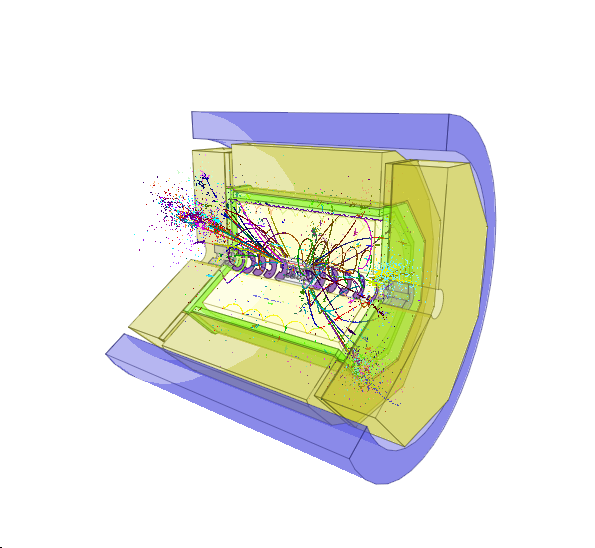
\includegraphics[width=0.8\textwidth]{img/title.png}\\[1cm]    
    \vfill
    % Bottom of the page
    %{\large Mai 2012}

    {\large 2012}
    
\end{center}
\end{titlepage}
\newpage

%\begin{abstract}
%test
%\end{abstract}

\tableofcontents
\newpage
\section{Introduction}
%\subsection{What CED is}
The C Event Display (CED) is a client server based tool to draw objects into a dynamic 3D picture. 
The client runs seperatly and connect to the server via a TCP/IP connection to send the objects which shall be drawn. 
%Although CED is able to send informations to the client. 
CED is a graphical application which uses OpenGL to display the 3D enviroment. 
It is possible to draw individual objects with CED (see section \ref{myviewer}) but for common use it is integrated into the ilcsoft framework.
The common use  is to display simulated events which happen in a particle collision. 
The recommended use is to read and process the datafile with \textit{Marlin} which, which sends the data of the events to CED. 
In order to do this, Marlin need a steering file. 
This steering file define which detector geometrie and which datafile is used and define which objects are drawn in which way.
Additional it configure which viewer are used, the viewer has a big impact in which way the event is displayed. 
Common viewers are: Generic-, CED- and DST-Viewer.
The steering file is formated in XML it can be created manual or generated automaticaly by MarlinGUI.
%The steering file decides which data file is read and also which viewer is used, the viewer decides which datatype is on what layer (see layer section), which color will be used etc. Example viewers are: Generic-, CED- and DST-Viewer.

%\subsection{(0.2 How do you get it)}
\section{Quickstart}
Generating a Marlin steering file can be time consumming, therefore there is a tool in the Marlin package which displays the event using a default configuration. 
For the first use, source the ini ilcsoft script and use the command: 
\begin{verbatim}
    ced2go <your datafile>
\end{verbatim}
A window which contains the graphical interpretation of your event will open. 
To view the next event press \textit{ENTER} in the terminal where you have commited the ced2go command.

\begin{figure}
    \begin{center}
         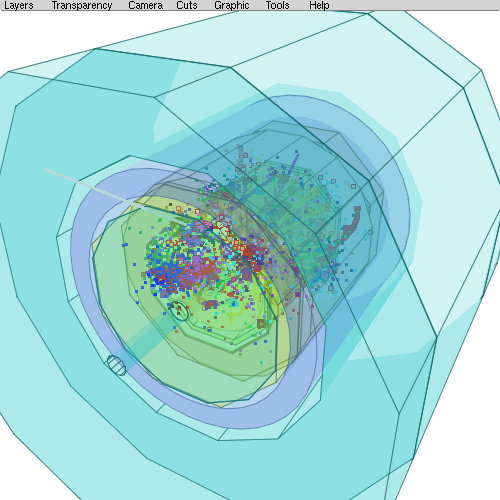
\includegraphics[width=0.5\linewidth]{img/quickstart.png}
         \caption{\label{CEDViewer} \textsl{ced2go after the first start}}
    \end{center}
\end{figure}

The generated Marlin steering file was written temporary at:
\begin{verbatim}
    /tmp/ced2go_<YOUR USER NAME>_steering.xml.  
\end{verbatim}
To configure Marlin one option is to modify this file and save it at a different location. 
To start CED manual and draw events with Marlin using the adjusted configuration file:
\begin{verbatim}
    glced&
    Marlin <YOUR STEERINGFILE>
\end{verbatim}


%All possible options are available from the menu at the top. 
%Additional you are able to use shortcuts (see appendix). 
%You are also able to change objects by the popup menu by clicking with the right mouse button at one object.



%\subsection{Help}
%Select the CED window and press 'h' to get an overlay of shortcuts and a description of used layers.

\subsection{CED Options}
There are three ways to interact and configure CED. 
By the main menu (at the top of the CED window), by the popup menu (right click into the CED window) or by keyboard.



\subsubsection{Main menu}
The main splitted into seven submenus: 
\begin{itemize}
    \item{Layers}: Toggle the visable of data or detector layers. 
    \item{Transparency}: Change the transparency of the detector components. 
    \item{Camera}: Change the possition of view, reset view or selecting projections. 
    \item{Cuts}: Different cuts of the detector. 
    \item{Graphic}: Graphic options. You can also save your prefered settings here.
    \item{Tools}: Additional functions like making high resolution screenshots.
    \item{Help}: Shows keyboard shortcuts.
\end{itemize}

\subsubsection{Popup menu}
Right-click on any object displayed in CED open the popup menu. 
This menu allows you to configure the selected object.
For example to change the color of the background simply click on it and chose a different one.
The popup menu differs for clicking at data, detector components or at the background.

\subsubsection{Keyboard shortcuts}
To display the available shortcuts use the shortcut 'h' (help), or select \textit{Help $\to$ Show keyboard shortcuts} from the main menu.
The available shortcuts are listed in section \ref{shortcuts}.

\subsubsection{Undo}
To undo the latest changes press ctrl+z.

\subsection{Save settings}
After changing the default options you are able to save the configuration for the next start. 
The settings are stored in \textit{$\sim$/.glced\_cfg/settings}.
The config file  is human readable but it is not recommended to change the settings by hand. 
Please notice that the current event or other Marlin settings are not saved, these depend only on the client. 

To save the settings select 
\textit{Graphic $\to$ Save settings $\to$ Save into slot $<$SLOT$>$} from the main menu. 
At the next start the setting which are saved in slot 1 are loaded automatical. 
To load annother configuration use 
\textit{Graphic $\to$ Load settings $\to$ Load settings $<SLOT>$}.


\section{Features}
\subsection{Rotate}
To change the view, simply left-click into the CED window, hold the mouse button and pull in any direction to rotate the view.
\subsection{Zoom factor}
To increase the magnification press '+', to decrease press '-'. If you are on Linux zooming with the mousewheel works too. 
Or use the main menu: \textit{Camera $\rightarrow$ Zoom in} and \textit{Camera $\rightarrow$ Zoom out}. 
%%here

\subsection{Move}
To move the center of the view to any direction, press and hold the middle mouse button and pull. 

To move in the direction of the y-axis, press arrow key $\uparrow$ or $\downarrow$. 
To move in the direction of the z-axis, press arrow key $\to$ or $\leftarrow$. 

\subsection{Center an object}
It is possible to center any data object drawn within CED. Simply put your mouse cursor over that object and press 'c' 

\subsection{Views}
\subsubsection{Side}
To view the detector from the side press 's', or choose it from the main menu under \textit{Camera $\to$ Side view}.

\subsubsection{Front}
To view the detector from front press 'f', or choose it from the main menu under \textit{Camera $\to$ Front view}.

\subsection{Projections}
There is a big difference between views and projections: View options show the same objects at a different angle, in contrast to projections which change the objects. 

\subsubsection{Side view projection}
\begin{figure}
\begin{minipage}[t]{6cm}
\centerline{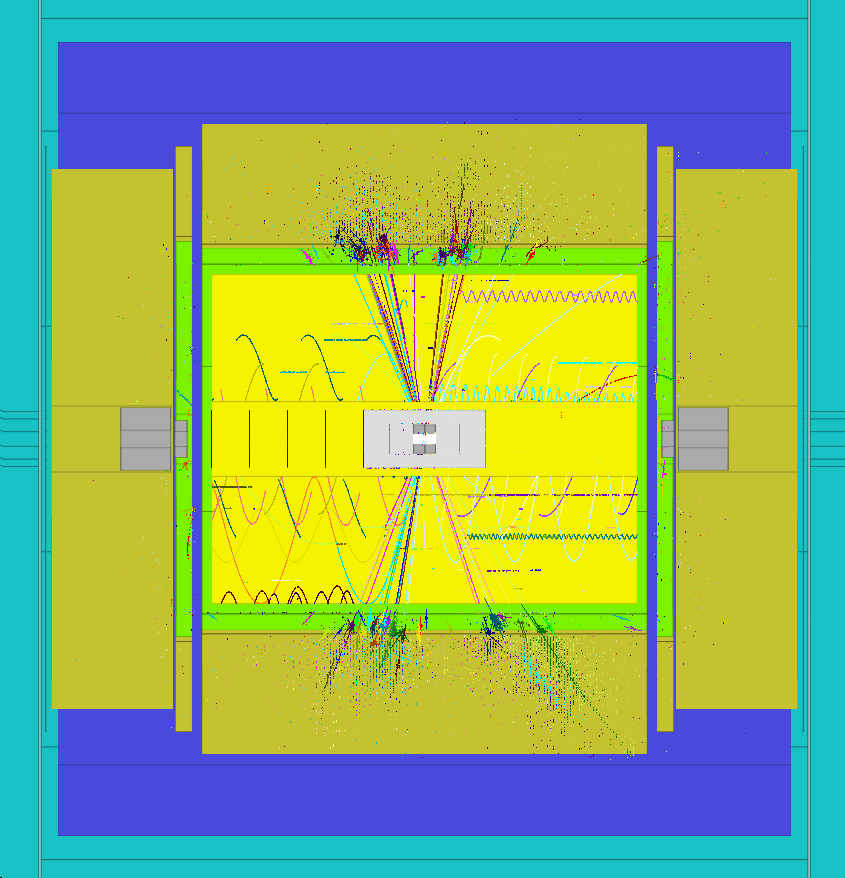
\includegraphics[height=5cm]{img/sideview.png}}
\caption{\label{CEDViewer} \textsl{Side view projection}}
\end{minipage}
\hfill
\begin{minipage}[t]{6cm}
\setlength{\fboxsep}{0mm}
\centerline{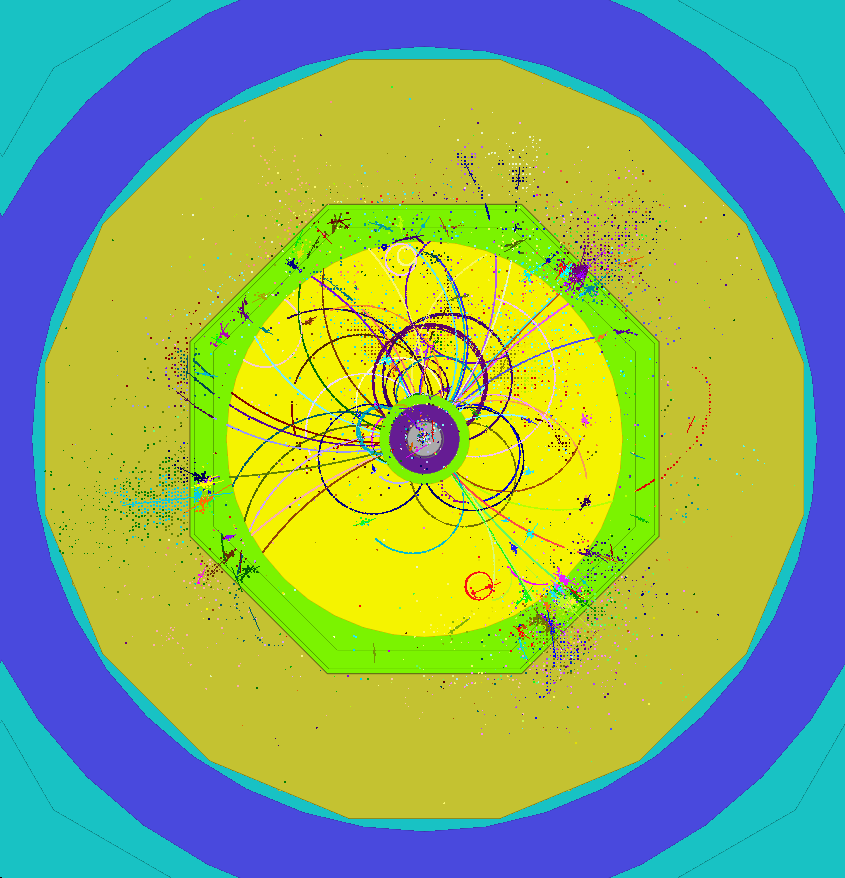
\includegraphics[height=5cm]{img/frontview.png}}
\caption{\label{DSTViewer}\textsl{Front view projection}}
\end{minipage}
\end{figure}


To enable side view projection press capital 'S', or choose it from the main menu under \textit{Camera $\to$ Toggle side view projection}. 
This projection turns the view into side view, and transforms all data (hits, tracks, etc) so that the distance from the beamline to the object are the same as in 3D mode.
\newline\newline
$y_{proj} = sign(y) \sqrt{x^2 + y^2}$\newline
$x_{proj}=0$\newline
$z_{proj} = z$ \newline
\newline
The detector is cut at $\phi=180$ to enable a view into it. The ability to rotate is  disabled. 
To exit this projection and get back to the previous view choose the side view projection mode again, or press 'S'. 




\subsubsection{Front view projection}
To enable front view projection press capital 'F', or choose it from the main menu under 
\textit{Camera $\to$ Toggle front view projection}.
This projection turns the view into front view, and transforms all data (hits, tracks etc)
($z_{proj} = 0$). The perspective is turned off and the detector is cut at z=0 to enable a view into the detector. The ability to rotate is disabled. To exit this projection, press 'F' or choose the front view projection mode again. 


\subsubsection{Fisheye view}
\begin{figure}
\centerline{ 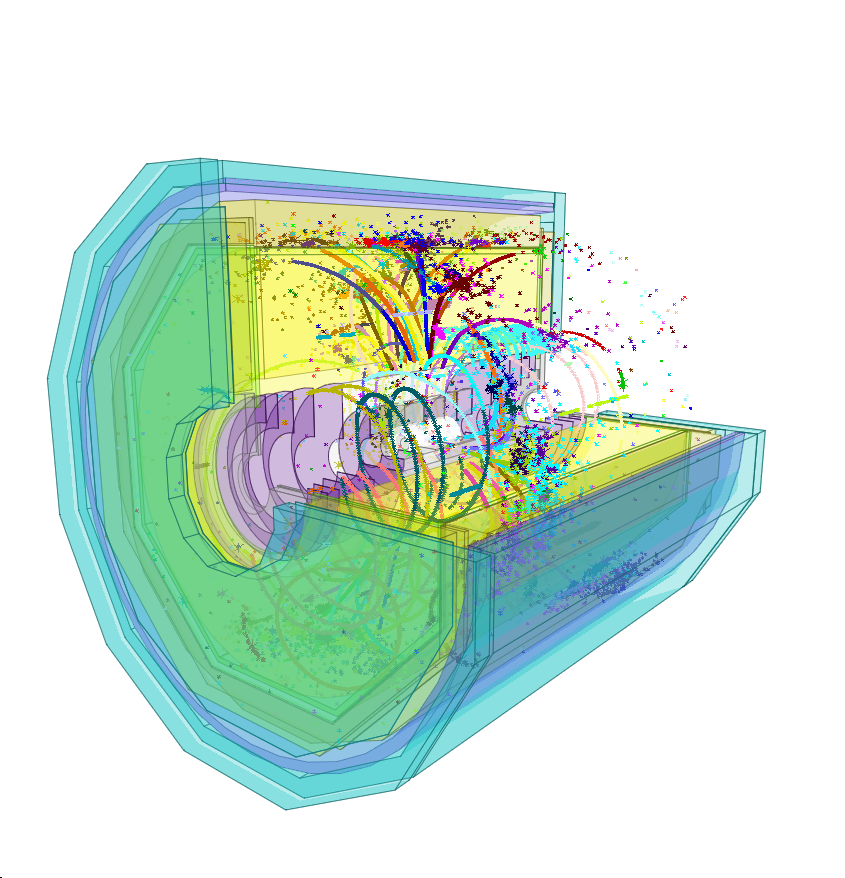
\includegraphics[height=8cm]{img/fisheye.png}}
\caption{\label{CEDViewer} \textsl{Fisheye projection (phi cut 90degree, transparency enabled)}}
\end{figure}

This projection enlarges the inner region of the detector, to give a clearer view to the inner tracks and hits of the event. To enable fisheye press 'v' or select it from the main menu under 
\textit{Camera $\rightarrow$ Toggle fisheye projection}. 
To turn this projection off, press 'v', or select it from the main menu again. The fisheye projection is usable together with the front or side view projection.


\subsection{Reset view settings}
To reset the view and cut settings press 'r', or choose it from the main menu under \textit{Camera $\rightarrow$ Reset view}. 
%This option resets: perspective, cutting, projections and zoom level.



\section{Layers}
It is possible to draw objects on different layers. 
This allows to show or hide specific types of data while working with CED. 
Both data and detector components are placed on layers. 
CED supports 100 different layers, but it is only possible to toggle the visibility of the first 25 data layers and the first 20 detector layers at runtime. 

\subsection{Data Layer}
To show which data is actually on which layer, open the overlaying help by pressing 'h', or choose \textit{Layers $\to$ Data layers} from the main  menu. 
To toggle the visibility of data layers quickly, there are shortcuts for the first 25 data layers. See section \ref{shortcuts}. 
Additional you are able to rightclick at any object and select \textit{Hide layer} to turn off the specific layer.
It is possible to turn all data layers simultaneously on or off by selecting \textit{Layers $\to$ Show/Hide all data layers}, or by pressing '$`$'

\subsection{Detector components}
Also detector components can be drawn on different layers. 
To toggle the visibility of detector components choose the corresponding component from \textit{Layer $\to$ Detector layers} in the main menu. 
It is possible to turn all components simultaneously on/off by selecting \textit{Layers $\to$ Show/Hide all detector components}. 

\begin{figure}
\centerline{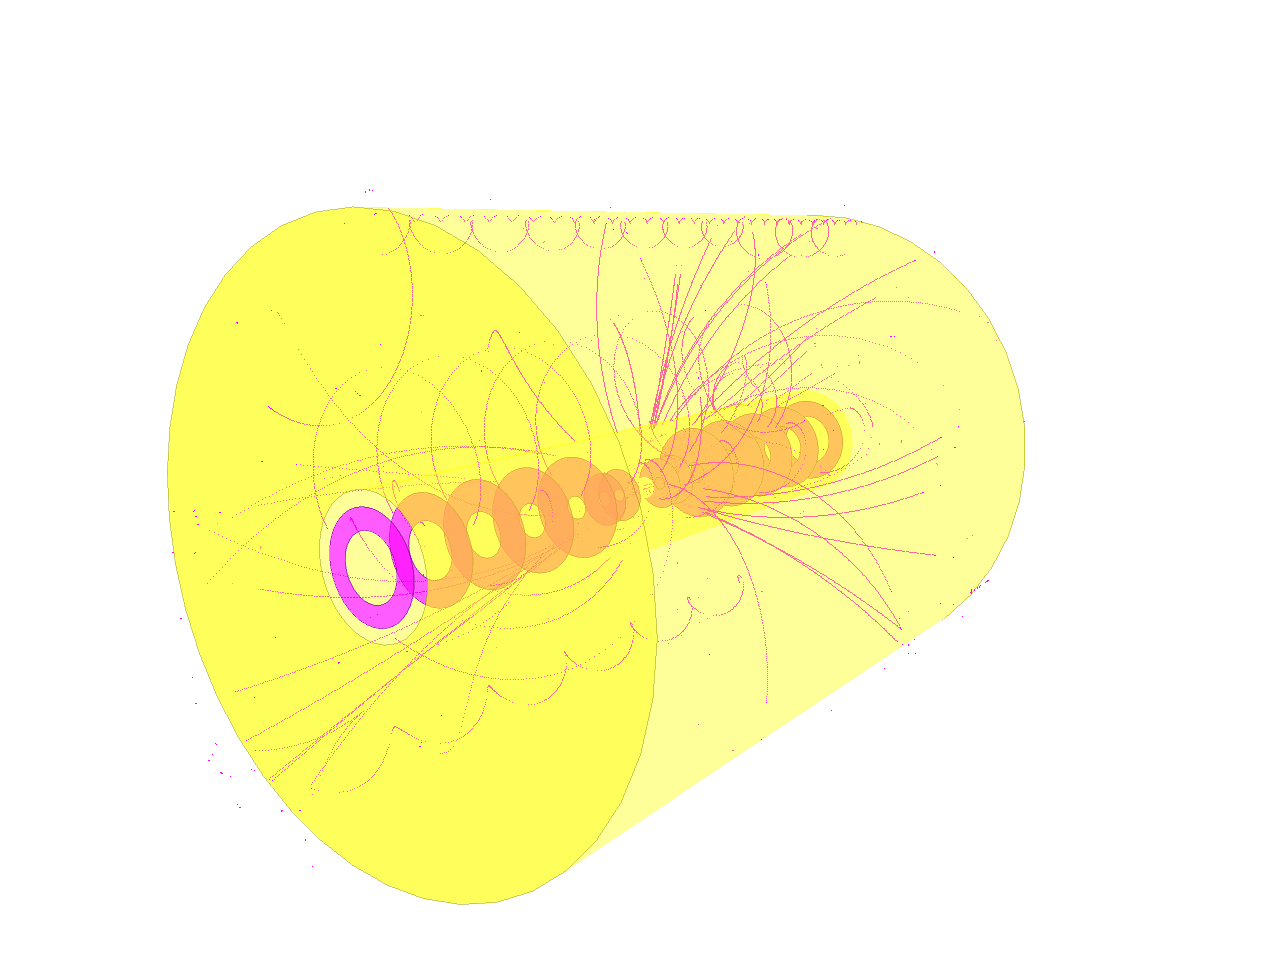
\includegraphics[height=6cm]{img/detector_layer.png}}
\caption{\label{detectorlayer} \textsl{Detector components: Some detector layers are turned off}}
\end{figure}

\section{Cuts}
In CED it is possible to cut a given range of $\phi$ out of the detector, or cut the detector at a specific z-axes value.

\subsection{Longitudinal cuts}
To cut down the detector in length select \textit{Cuts $\to$ Cut at z=$<$VALUE$>$} from the main menu.
To cut one component seperatly rightclick on this component (detector picking must be enabled) and select \textit{Z-cut $\to$ cut at z=$<$VALUE$>$}. 
To cut the detector stepless press and hold capital 'Z' to enlarge the detector back, press and hold 'z'.
This feature affects all detector components simulatanly if no component is selected, when one component is selected only the selected one is modified.

\begin{figure}
\begin{minipage}[t]{6cm}
\centerline{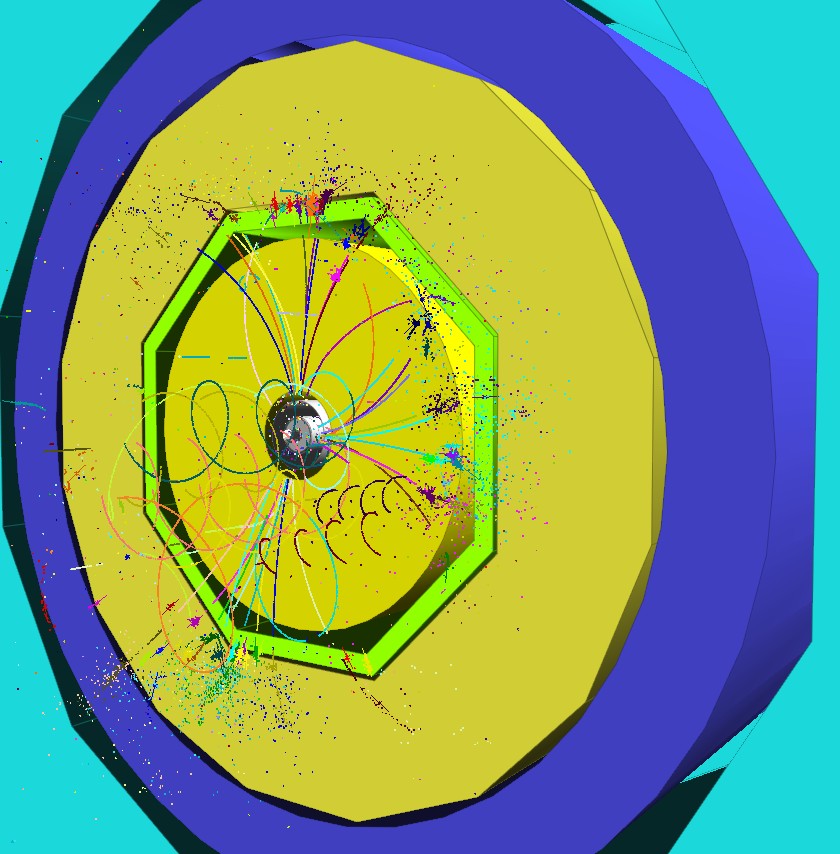
\includegraphics[width=0.8\textwidth]{img/zcut.png}}
\caption{\label{CEDViewer} \textsl{Longitudinal cut (z=0, lightning enabled)}}
\end{minipage}
\begin{minipage}[t]{6cm}
\setlength{\fboxsep}{0mm}
\centerline{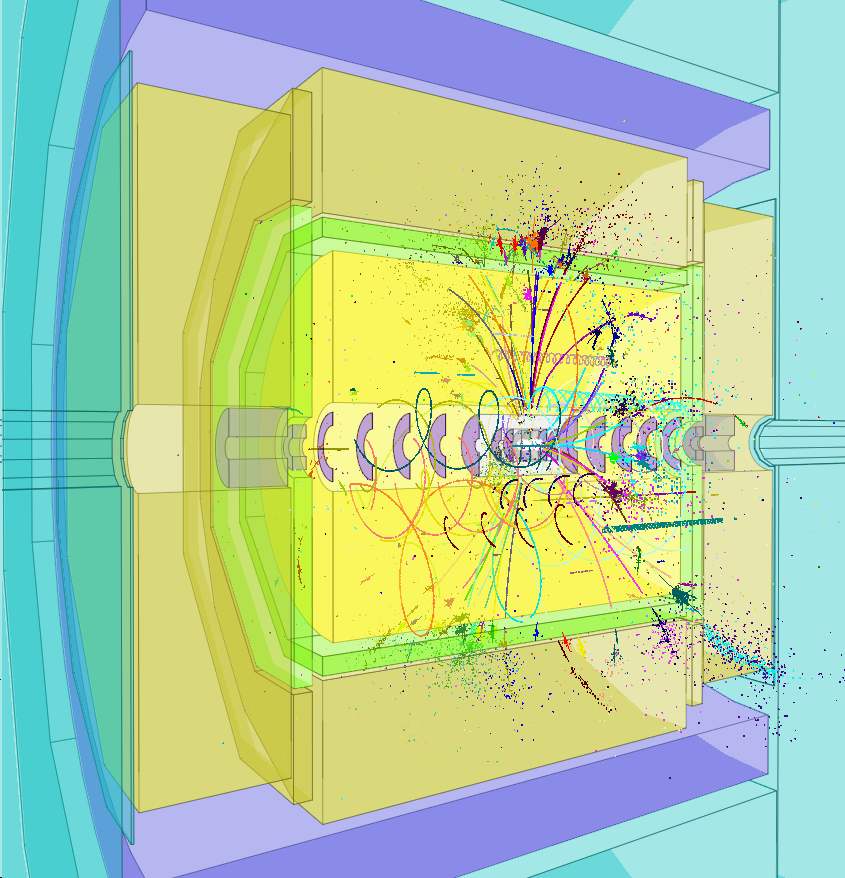
\includegraphics[width=0.8\textwidth]{img/phicut.png}}
\caption{\label{DSTViewer}\textsl{Phi cut ($\phi$=90 degree, transparency enabled)}}
\end{minipage}
\end{figure}



\subsection{Phi cuts}
To cut down the detector in $\phi$ select \textit{Cuts $\to$ Cut at phi=$<VALUE>$} from the main menu.
To cut one component seperatly rightclick on this component (detector picking must be enabled) and select \textit{Phi-cut $\to$ cut at phi=$<VALUE>$}. 
To cut the detector stepless press and hold capital 'M' to enlarge the detector back, press and hold 'm'.
This feature affects all detector components simulatanly if no component is selected, when one component is selected only the selected one is modified.




\section{Background color}
\begin{figure}
\begin{minipage}[t]{6cm}
\centerline{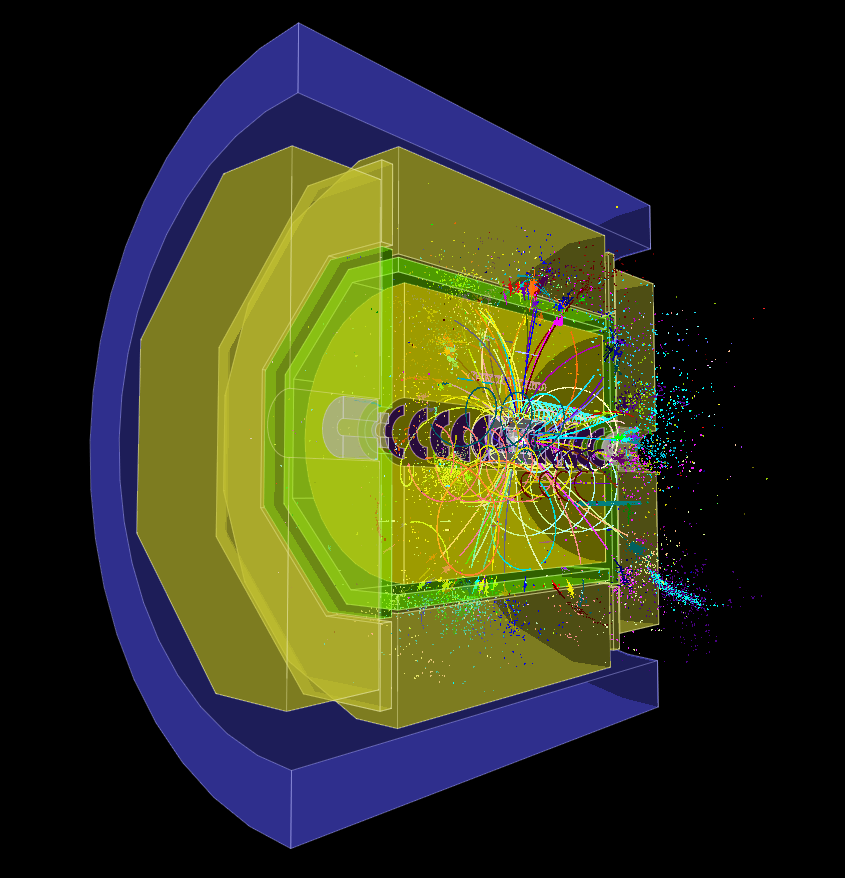
\includegraphics[width=0.8\textwidth]{img/black.png}}
\caption{\label{CEDViewer} \textsl{Background color: black (transparency enabled, phi cut)}}
\end{minipage}
\hfill
\begin{minipage}[t]{6cm}
\setlength{\fboxsep}{0mm}
\centerline{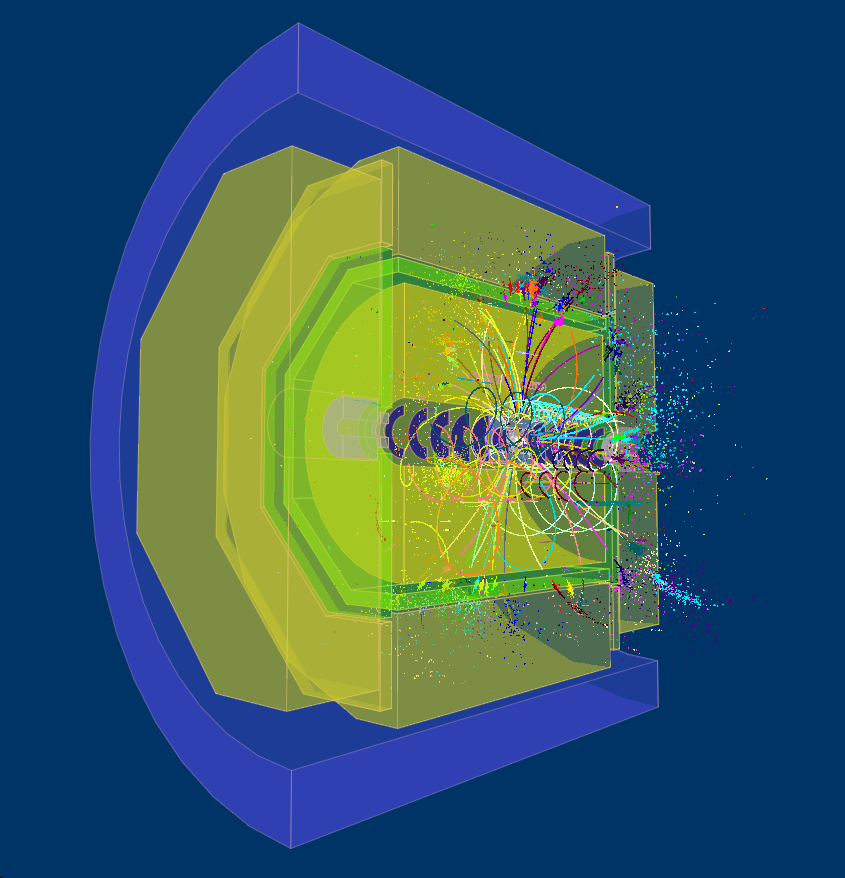
\includegraphics[width=0.8\textwidth]{img/blue.png}}
\caption{\label{User viewer}\textsl{Background color: blue (transparency enabled, phi cut)}}
\end{minipage}
\end{figure}

Changing the background color is not only a setting to increase the aesthetic of the picture, it can also be used to increase the visiblility of the drawn data.
To toggle the background color select \textit{Graphic $\to$ Change background color $\to$ $<$COLORNAME$>$} from the main menu or right-click at a free place in the in the CED window and select one of the colornames in the popup menu.  
Another way is to use the shortcut 'b' to change the background color from blue to black, over gray to white.
To add an induvidual color you are able to add a color code at the startup time. 
For example to add the color 0xFF0000: 
\begin{verbatim}
  glced -bgcolor FF0000 
\end{verbatim}
When another background color is loaded from your setting file you can press 'b' several times until your user defined background color appears. 
After that you are able to save this color by save your settings. 



%\begin{figure}[h]
%\begin{minipage}[t]{6cm}
%\centerline{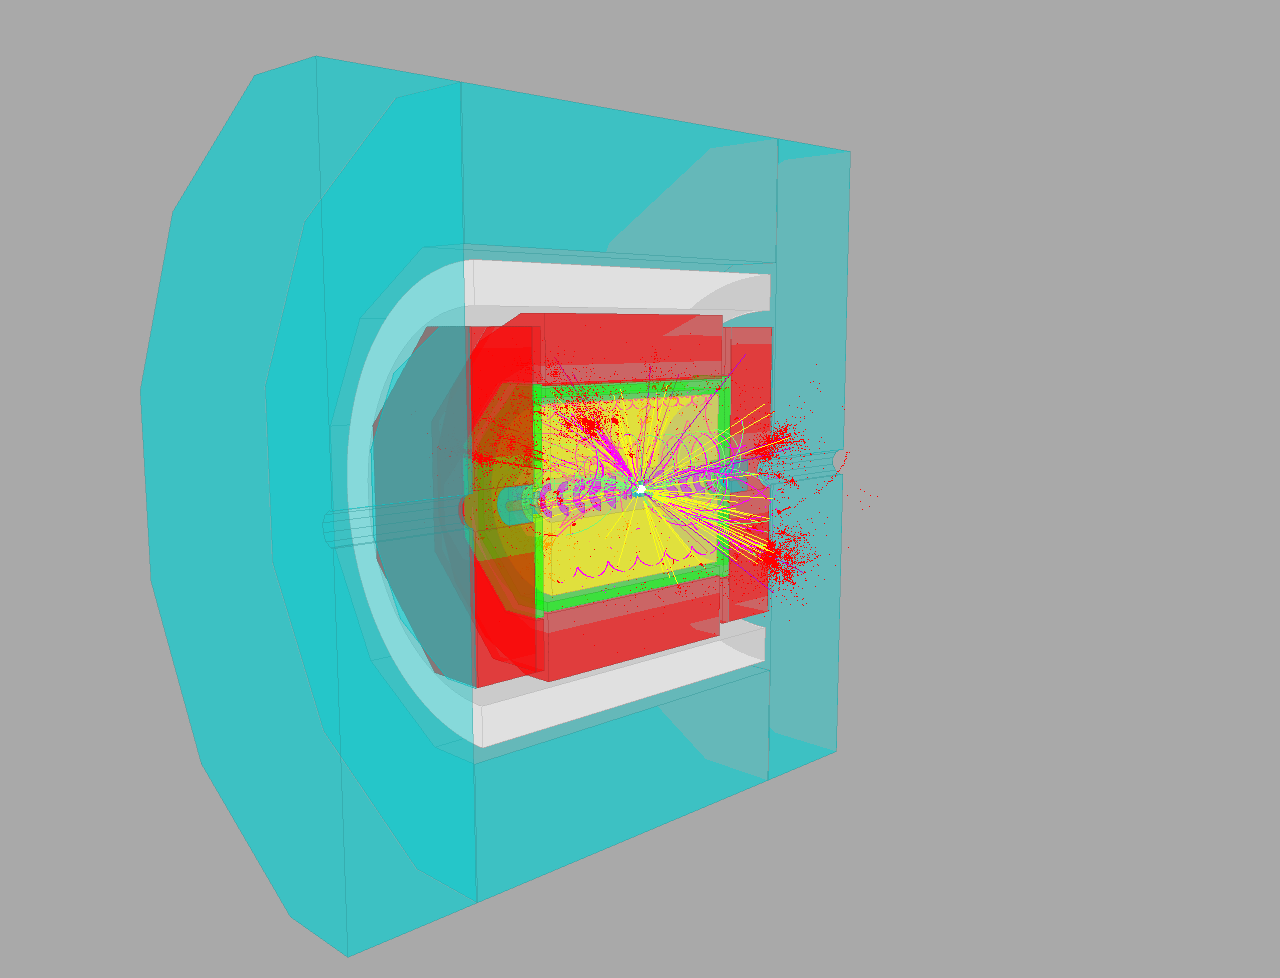
\includegraphics[height=4.5cm]{bg_color_dackgray1.png}}
%\caption{\label{CEDViewer} \textsl{Background color: darkgray}}
%\end{minipage}
%\hfill
%\begin{minipage}[t]{6cm}
%\setlength{\fboxsep}{0mm}
%\centerline{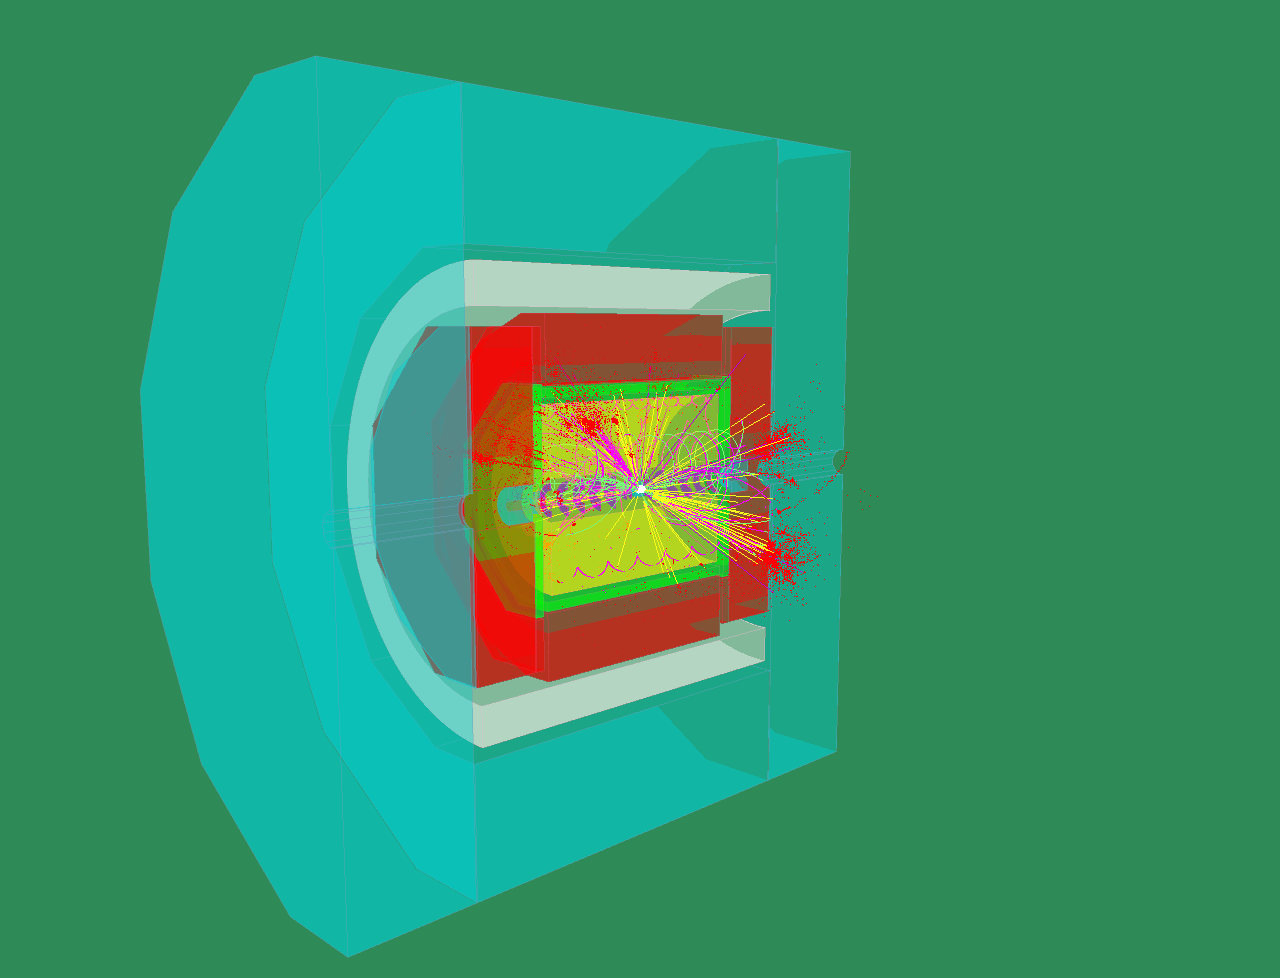
\includegraphics[height=4.5cm]{bg_color_green1.png}}
%\caption{\label{DSTViewer}\textsl{Background color: green}}
%\end{minipage}
%\end{figure}
%

For some examples colorcodes see figure \ref{html}.
\begin{figure}
\setlength{\fboxsep}{0mm}
\centerline{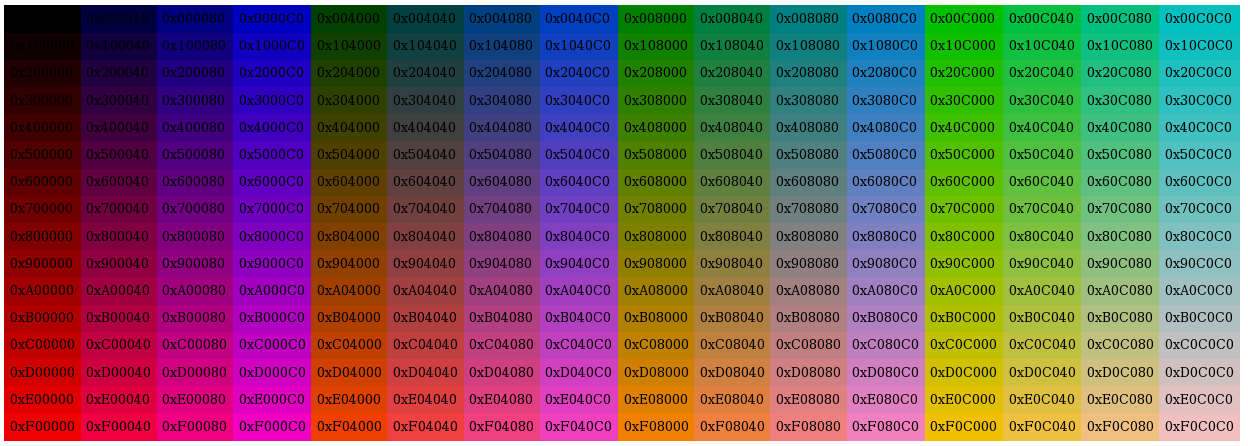
\includegraphics[width=1\linewidth]{img/html_colors.png}}
\caption{\label{html}\textsl{Some HTML color codes}}
\end{figure}

\section{Graphical options}
\subsection{Classic and new view}
To toggle between classic and new view chose 'Graphics options $\rightarrow$ Graphic low' or 'Graphics options $\rightarrow$ Graphic high' from the main menu. There are two graphical settings which are affected by this option:
 \begin{center}
 \begin{tabular}[ht]{|l|c|c|}
  \hline
  &Graphic low & Graphic high\\
  \hline
  Detector look & mesh & transparency\\
  Perspective & flat & 3D\\
  \hline
\end{tabular}
\end{center}

\begin{figure}
\begin{minipage}[t]{6cm}
\setlength{\fboxsep}{0mm}
\centerline{\fbox{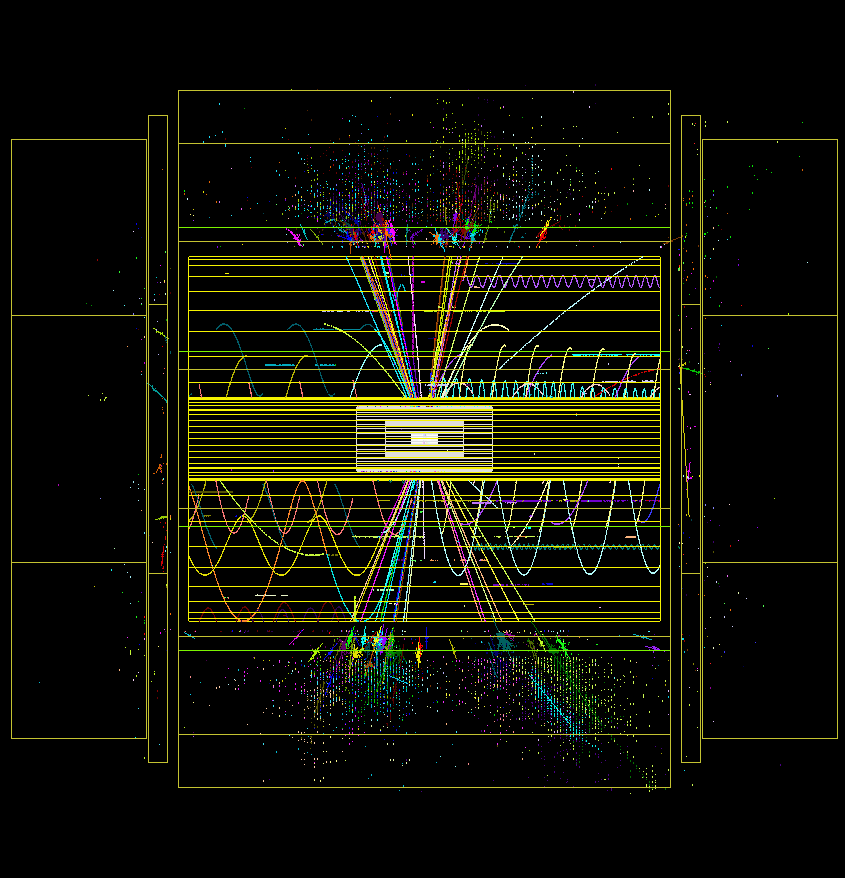
\includegraphics[width=0.8\textwidth]{img/classic.png}}}
\caption{\label{CEDViewer} \textsl{Classic view. (Side projection, black background)}}
\end{minipage}
\hfill
\begin{minipage}[t]{6cm}
\setlength{\fboxsep}{0mm}
\centerline{\fbox{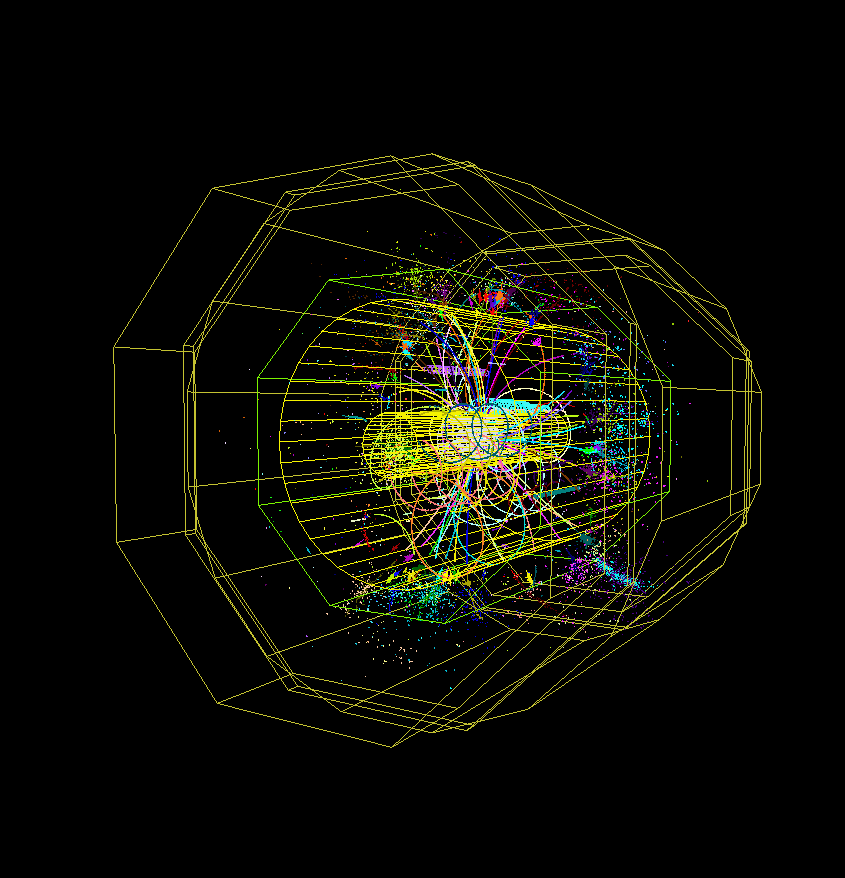
\includegraphics[width=0.8\textwidth]{img/classic2.png}}}
\caption{\label{DSTViewer}\textsl{Mesh view (perspective enabled, black background)}}
\end{minipage}
\end{figure}


\subsection{Perspective setting}
To turn the perspective on or off, select 'Graphic $\rightarrow$ Toggle perspective' from main menu. 
Objects which are further away from the viewer appear smaller when perspectiv view is enabled, otherwise all objects appear in the same size.

\subsection{Transparency and mesh view}
To change the way the detector is drawn, select \textit{Graphic $\rightarrow$ Toggle wireframe} from main menu.
\subsection{Visibility of coordinate axes}
Per default at the point (0, 0, 0) the kartesian axis are shown.
To turn axis off select \textit{Layer $\rightarrow$ Axis} from the main menu.

%\begin{center}
%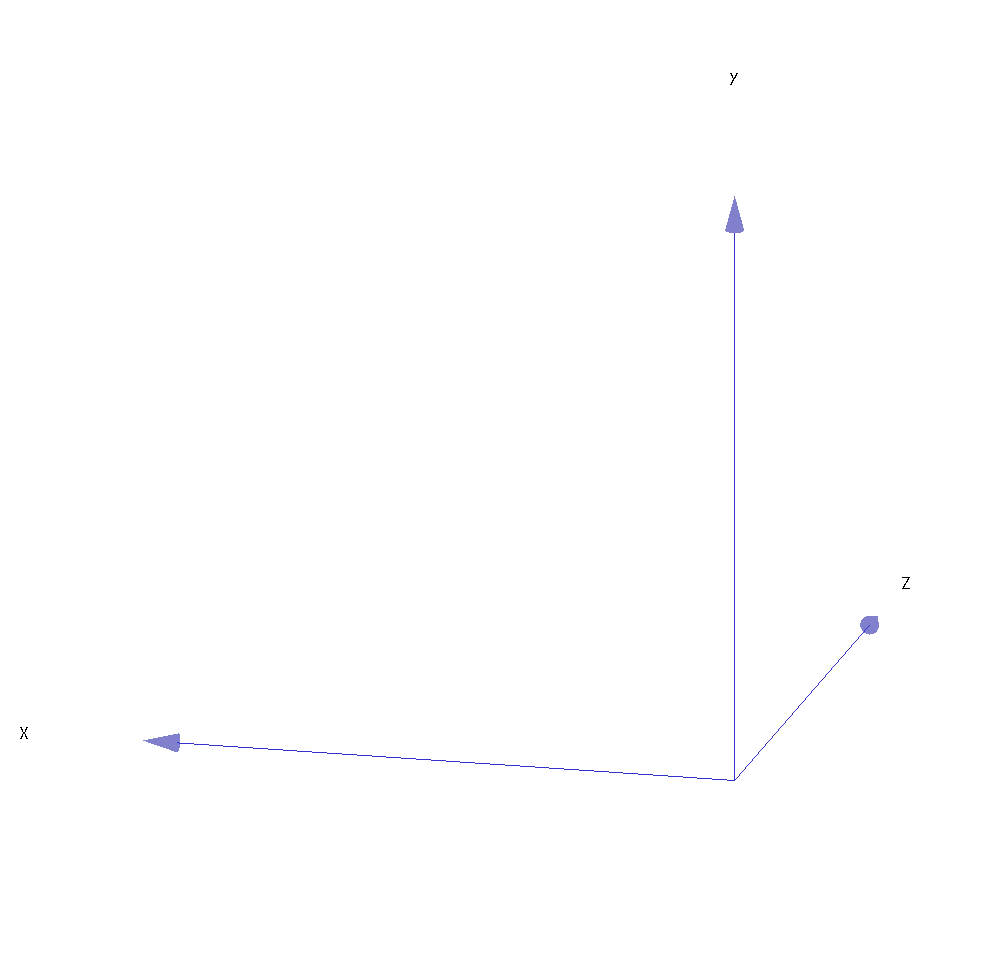
\includegraphics[width=4cm]{axes1.png}
%\end{center}

\subsection{Transparency value}
While not in mesh view, it is possible to change the value of detector transparency by selecting \textit{Transparency $\rightarrow$ $<$VALUE$>$\%} from main menu. 
Possible values are: 0, 40, 60, 70, 80, 90, 95 and 100\%.
To adjust the transparency stepless use the shortcut keys '$>$' and '$<$'. 
When selecting a detector component first only the selected component is modified. 
Additional it is possible to rightclick at an detector component and select \textit{Transparency $\to$ $<$VALUE$>$\%} from the popup menu.


%\begin{figure}[h!]
%\begin{minipage}[t]{6cm}
%\setlength{\fboxsep}{0mm}
%\centerline{\fbox{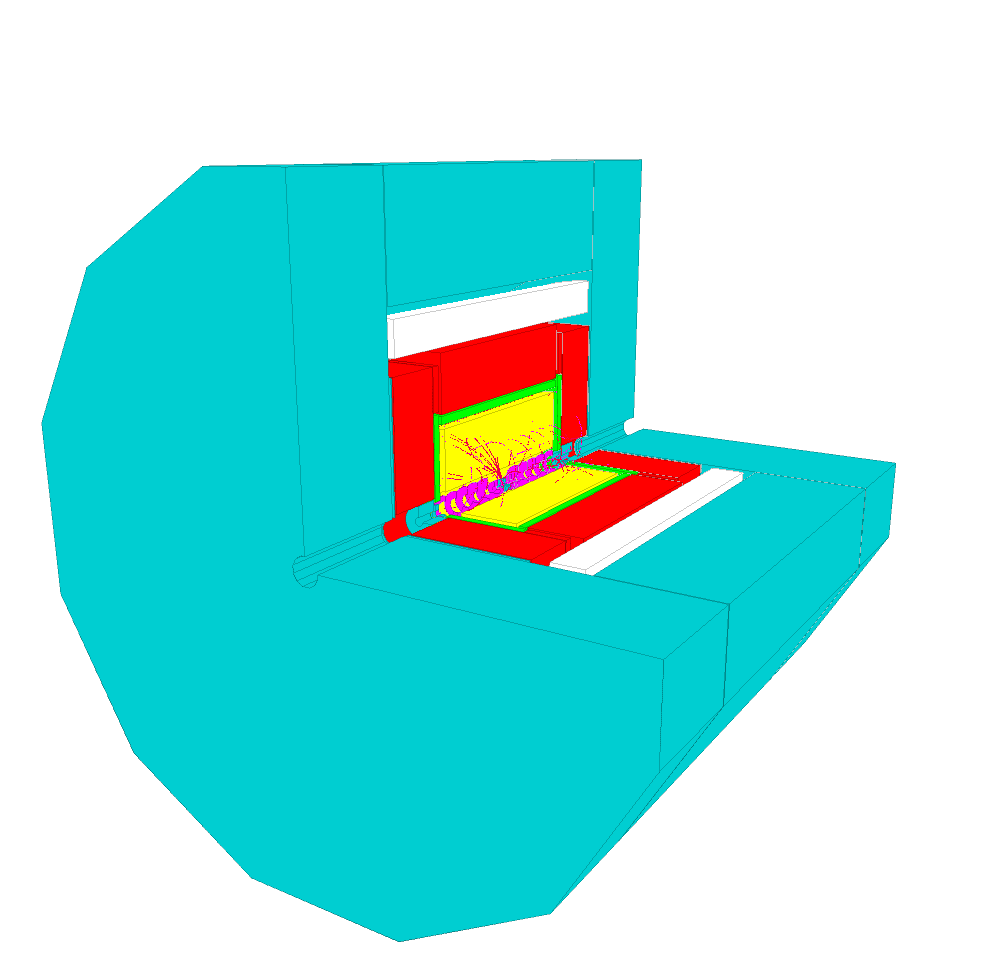
\includegraphics[height=5.5cm]{transparency_0.png}}}
%\caption{\label{CEDViewer} \textsl{Transparency 0\%}}
%\end{minipage}
%\hfill
%\begin{minipage}[t]{6cm}
%\setlength{\fboxsep}{0mm}
%\centerline{\fbox{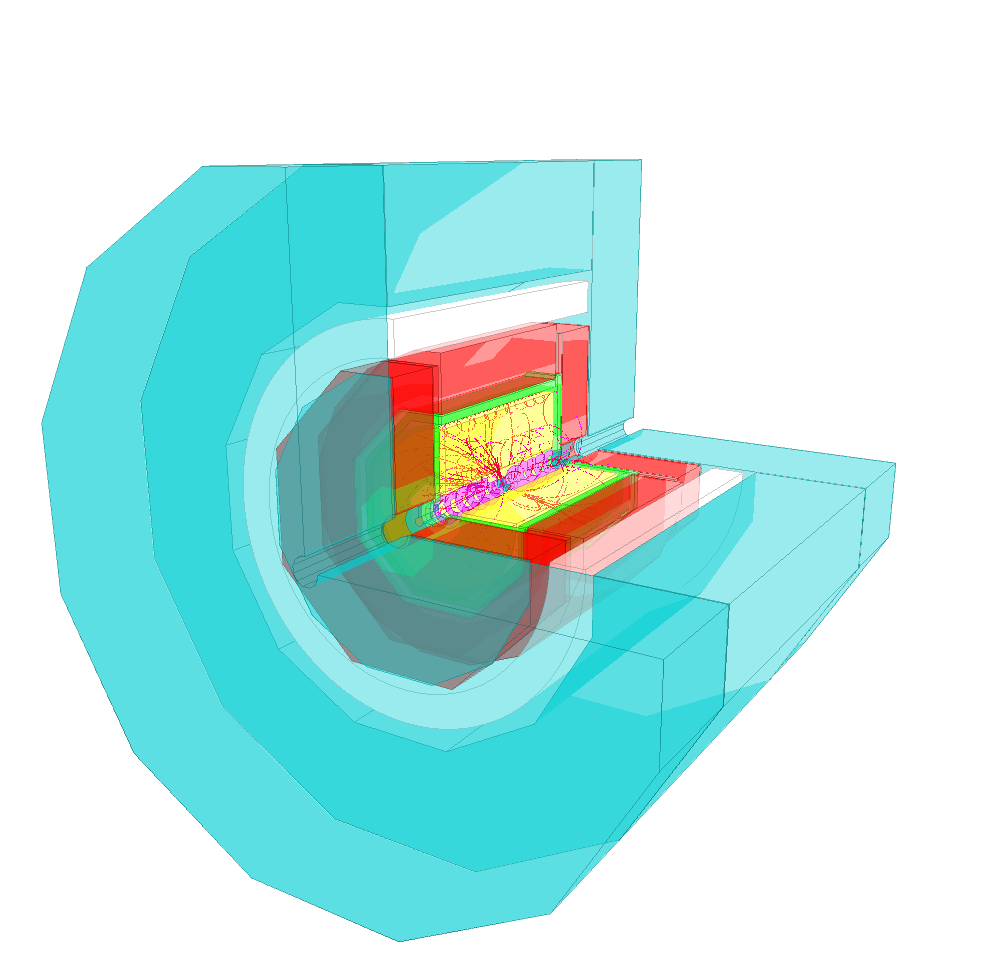
\includegraphics[height=5.5cm]{transparency_60.png}}}
%\caption{\label{DSTViewer}\textsl{Transparency 60\%}}
%\end{minipage}
%\end{figure}
%
%\begin{figure}[h!]
%\begin{minipage}[t]{6cm}
%\setlength{\fboxsep}{0mm}
%\centerline{\fbox{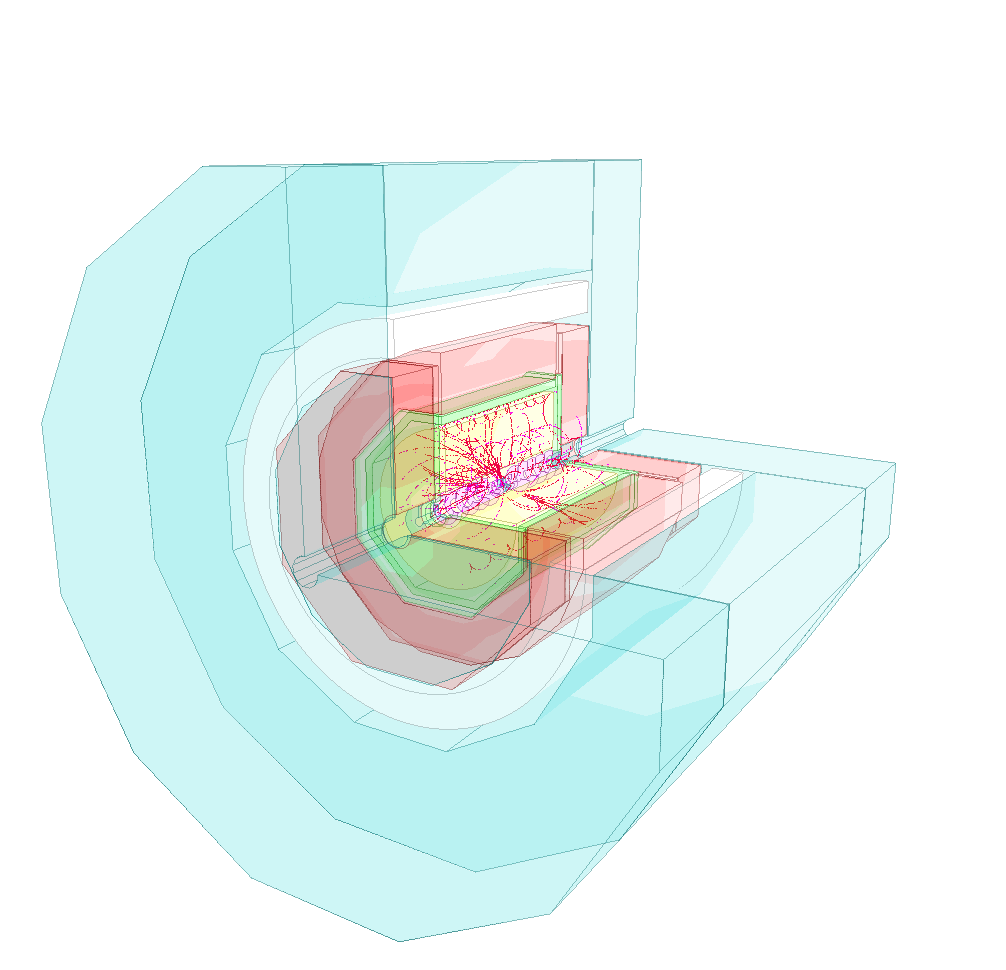
\includegraphics[height=5.5cm]{transparency_90.png}}}
%\caption{\label{CEDViewer} \textsl{Transparency 90\%}}
%\end{minipage}
%\hfill
%\begin{minipage}[t]{6cm}
%\setlength{\fboxsep}{0mm}
%\centerline{\fbox{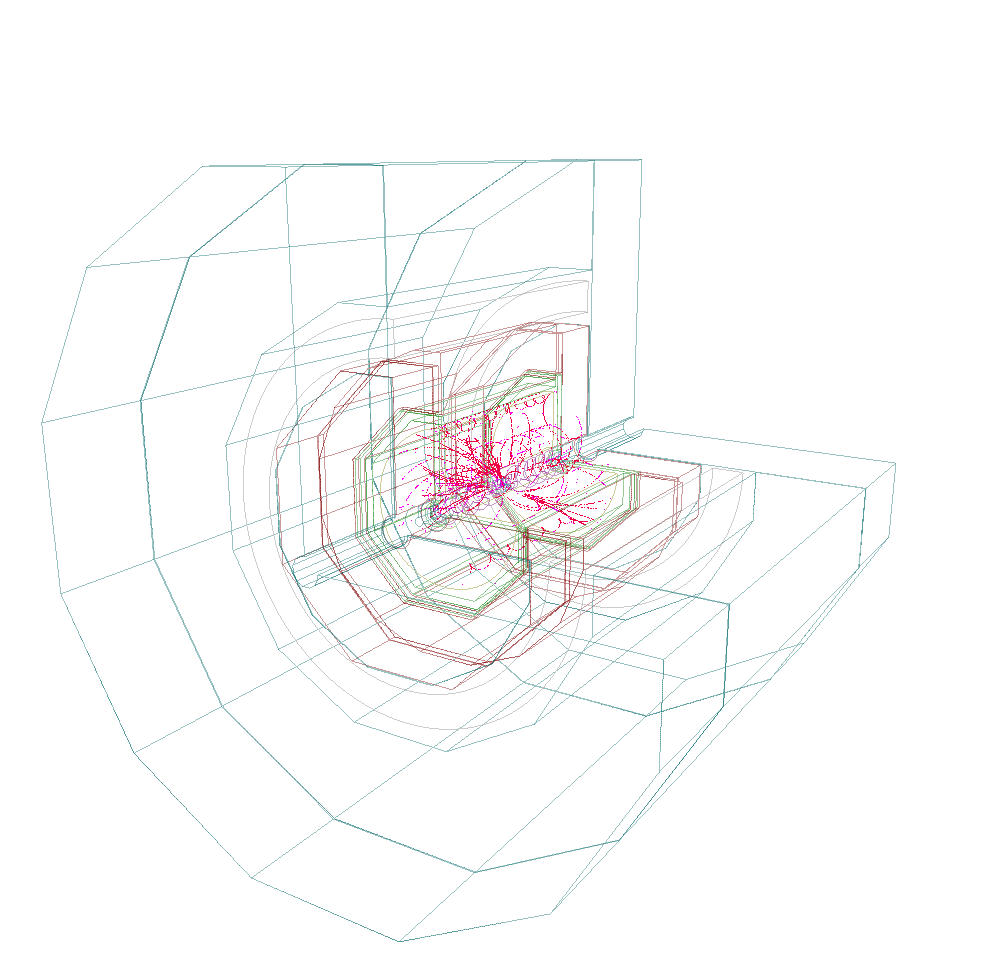
\includegraphics[height=5.5cm]{transparency_100.png}}}
%\caption{\label{DSTViewer}\textsl{Transparency 100\%}}
%\end{minipage}
%\end{figure}


\subsection{Light}
To enable lightning select \textit{Graphic $\to$ Light} from the main menu.

\subsection{Fog}
To enable Fog select \textit{Graphic $\to$ Fade far objects} from the main menu.
This mode fades far objects into the current background color.
Notice that the applied fade color does not change after changing the background color. 
If you like to update the color select this option twice.


\subsection{Frames per seconds}
To measure the performance of CED, there is a build-in function called Frames per seconds (FPS). 
Normaly CED only renders a new image after changes, such as toggleing the visibility of a layer, or changing the view. 
In contrast, in FPS mode CED renders so many images as possible and prints out, how many images there were rendered in the last second. 
This allows, to compare the performance of CED in different circumstances, for instance different versions, different viewers, or different machines. 

\section{Picking}
Double click on the object in which you are interested in, Marlin will print out information about the selected object. 
Another way is to rightclick at the object and select \textit{Pick object} from the popup menu. 

\begin{figure}[h!]
\begin{minipage}[t]{6cm}
\setlength{\fboxsep}{0mm}
\centerline{\fbox{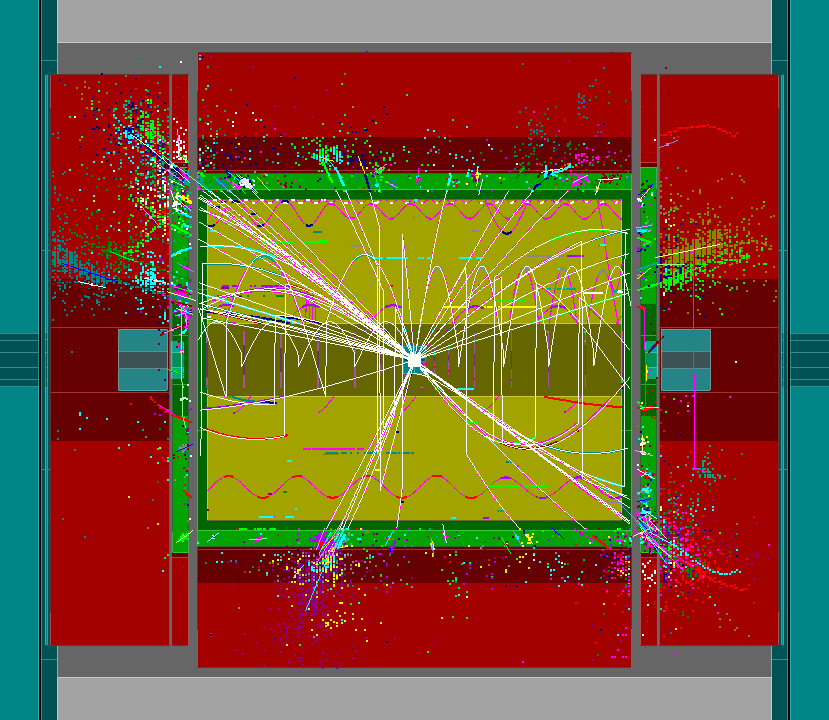
\includegraphics[height=5cm]{img/picking_ced_window.png}}}
\caption{\label{CEDViewer} \textsl{CED window}}
\end{minipage}
\hfill
\begin{minipage}[t]{6cm}
\setlength{\fboxsep}{0mm}
\centerline{\fbox{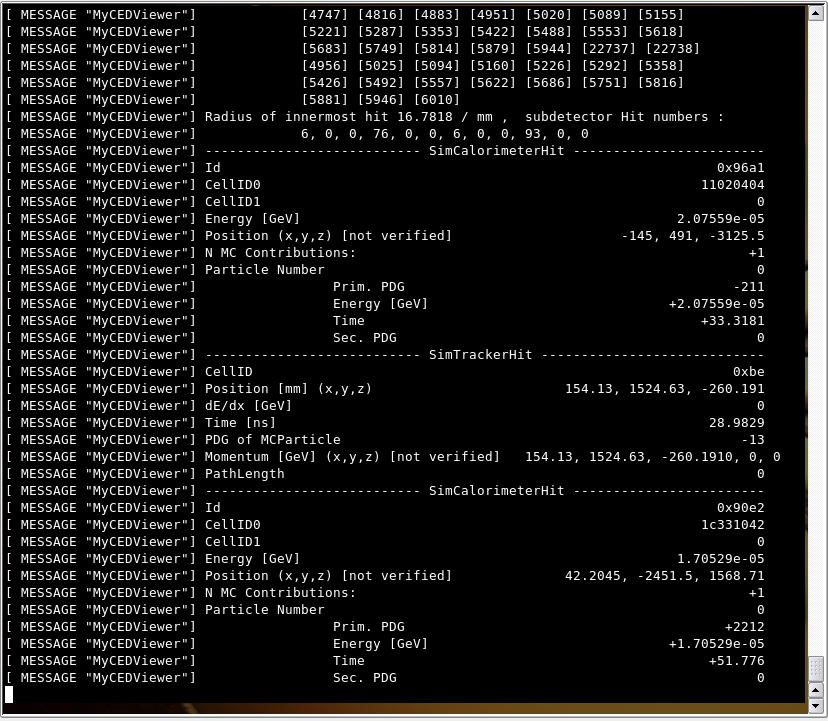
\includegraphics[height=5cm]{img/picking_terminal_window.png}}}
\caption{\label{DSTViewer}\textsl{Terminal where Marlin runs}}
\end{minipage}
\end{figure}
 
\section{Screenshot}
To create a high resolution screenshot select \textit{Tools $\to$ Save screenshot $\to$ $<$SIZE$>$} from the main menu. 
The screenshot is saved in the TGA format in the current location where CED was started as \textit{glced-N.tga} where $N$ starts from 1 and gets increased
with the number of saved screenshots. Converting the screenshot into for example png use:
 \begin{verbatim}
      convert glced.tga screenshot.png
 \end{verbatim}
or in batch mode
\begin{verbatim}
      for i in `ls -1 glced-*.tga`;
      do
        convert $i `basename $i .tga`.png;
      done
 \end{verbatim}
 
\section{Viewer}
To draw an event with Marlin into CED, Marlin needs a configuration file, written in XML. This file is called the Marlin-Steeringfile, see its documentation for details. In this file one or more viewers are configured. There a a number of different viewers available in ilcsoft: CEDViewer, DSTViewer, Generic Viewer, and Vertex Viewer. The difference between these viewers is how the event gets drawn. The detector geometry does not depend on with viewer is used. 

A sample viewer configuration section could be:
 \begin{verbatim}
  <execute>
      <processor name="MyGenericViewer"/>
   </execute>

 <processor name="MyGenericViewer" type="GenericViewer">
   <!--Sim Calo Hit Collection Names-->
   <parameter name="SimCaloHitCollections" type="StringVec"
        lcioInType="SimCalorimeterHit"> 
        BeamCalCollection EcalBarrelCollection
        EcalBarrelPreShowerCollection EcalEndcapCollection 
        EcalEndcapPreShowerCollection EcalEndcapRingCollection 
        EcalEndcapRingPreShowerCollection HcalBarrelRegCollection 
        HcalEndCapRingsCollection HcalEndCapsCollection LHcalCollection 
        LumiCalCollection MuonEndCapCollection 
   </parameter>
   
   <!--Sim Tracker Hit Collection Names-->
   <parameter name="SimTrackerHitCollections" type="StringVec" 
        lcioInType="SimTrackerHit"> 
        ETDCollection FTDCollection SETCollection SITCollection 
        TPCCollection TPCSpacePointCollection VXDCollection 
   </parameter>

   <!--Layer for Sim Calo Hits-->
   <parameter name="LayerSimCaloHit" type="int" value="5"/>
   
   <!--Layer for Sim Tracker Hits-->
   <parameter name="LayerSimTrackerHit" type="int" value="6"/>
</processor>

 \end{verbatim}
A viewer is used from Marlin as a library and to specify the style, color and layer of things which are drawn into CED.

Examples of different viewers are shown in Figure \ref{CEDViewer} - \ref{User viewer}. 

\begin{figure}[h]
\begin{minipage}[t]{6cm}
\setlength{\fboxsep}{0mm}
\centerline{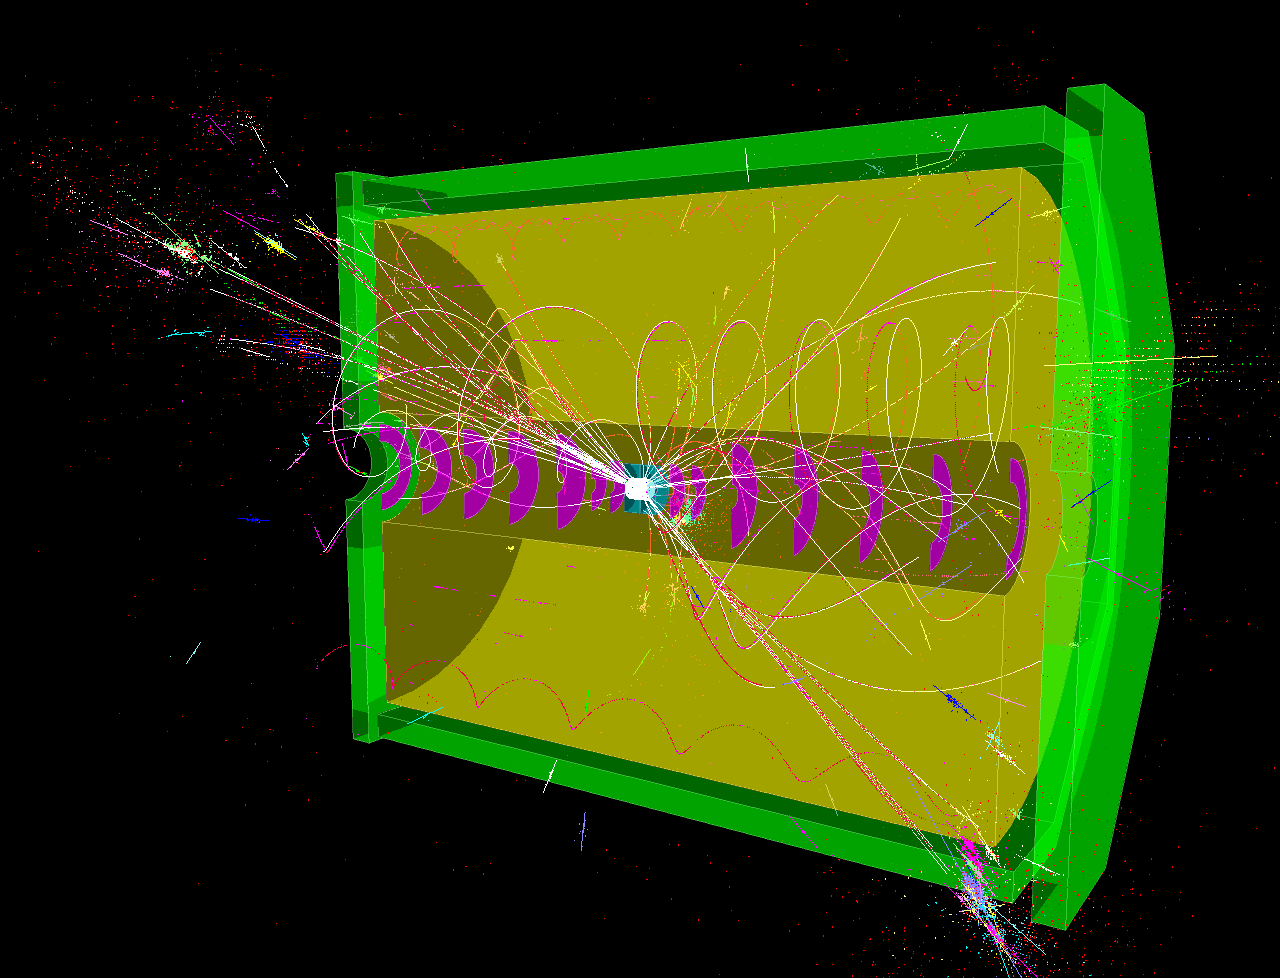
\includegraphics[height=4.4cm]{img/ced_viewer.png}}
\caption{\label{CEDViewer} \textsl{CEDViewer}}
\end{minipage}
\hfill
\begin{minipage}[t]{6cm}
\setlength{\fboxsep}{0mm}
\centerline{\fbox{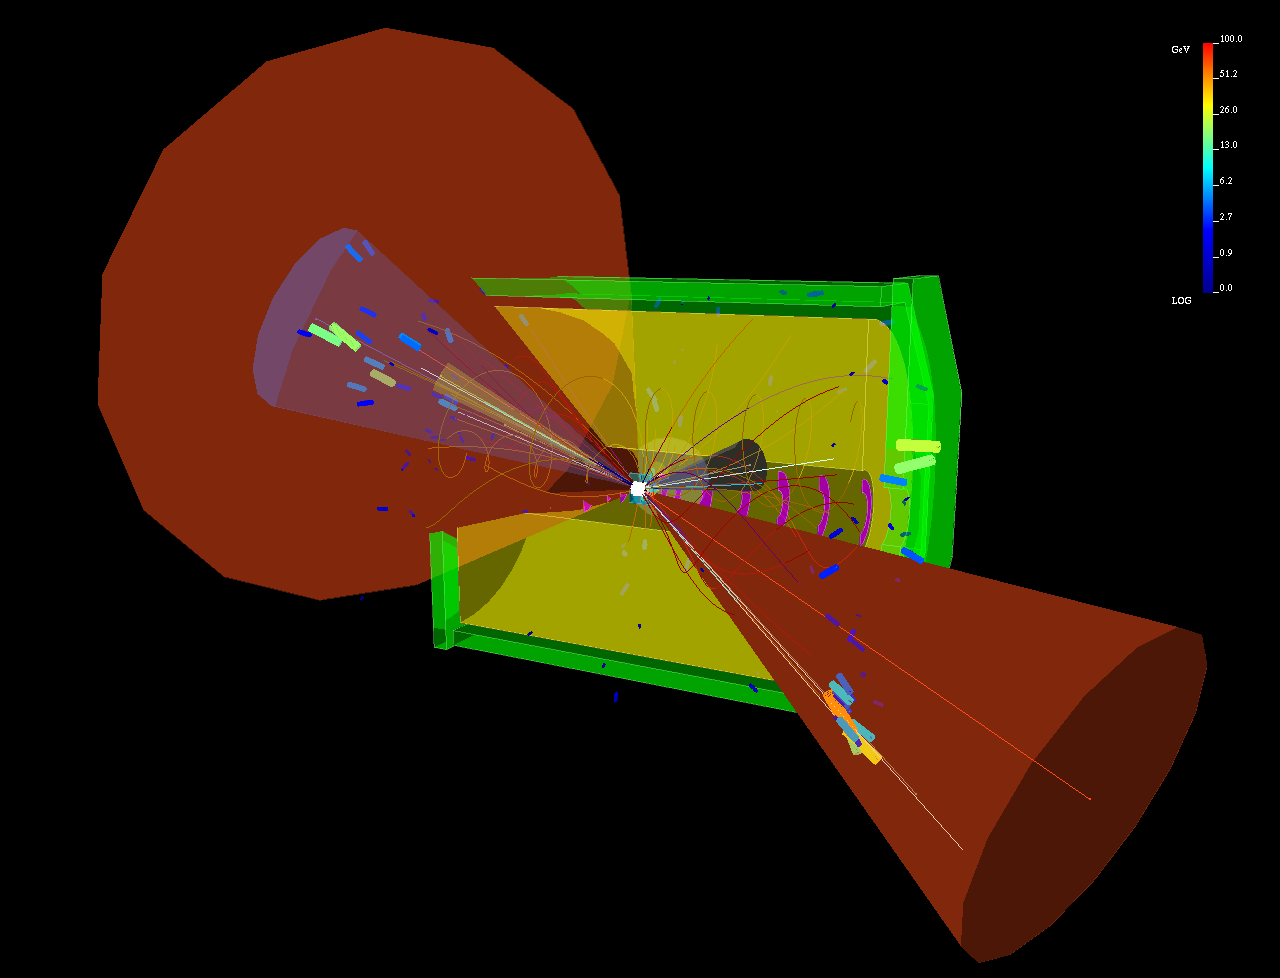
\includegraphics[height=4.4cm]{img/dst_viewer.png}}}
\caption{\label{DSTViewer}\textsl{DSTViewer}}
\end{minipage}
\end{figure}

\begin{figure}[h]
\begin{minipage}[t]{6cm}
\setlength{\fboxsep}{0mm}
\centerline{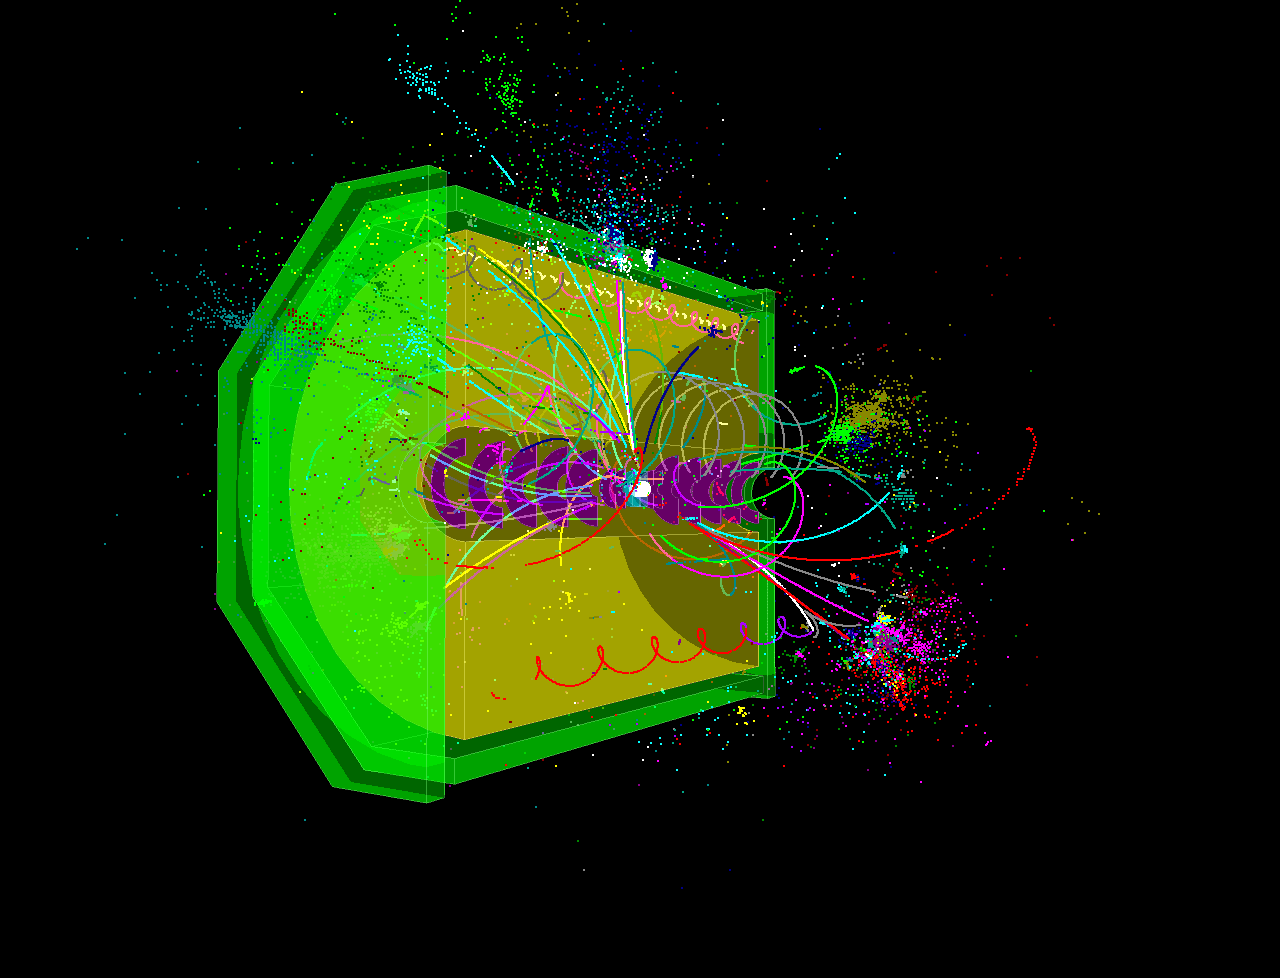
\includegraphics[height=4.4cm]{img/generic_viewer.png}}
\caption{\label{GenericViewer} \textsl{GenericViewer}}
\end{minipage}
\hfill
\begin{minipage}[t]{6cm}
\setlength{\fboxsep}{0mm}
\centerline{\fbox{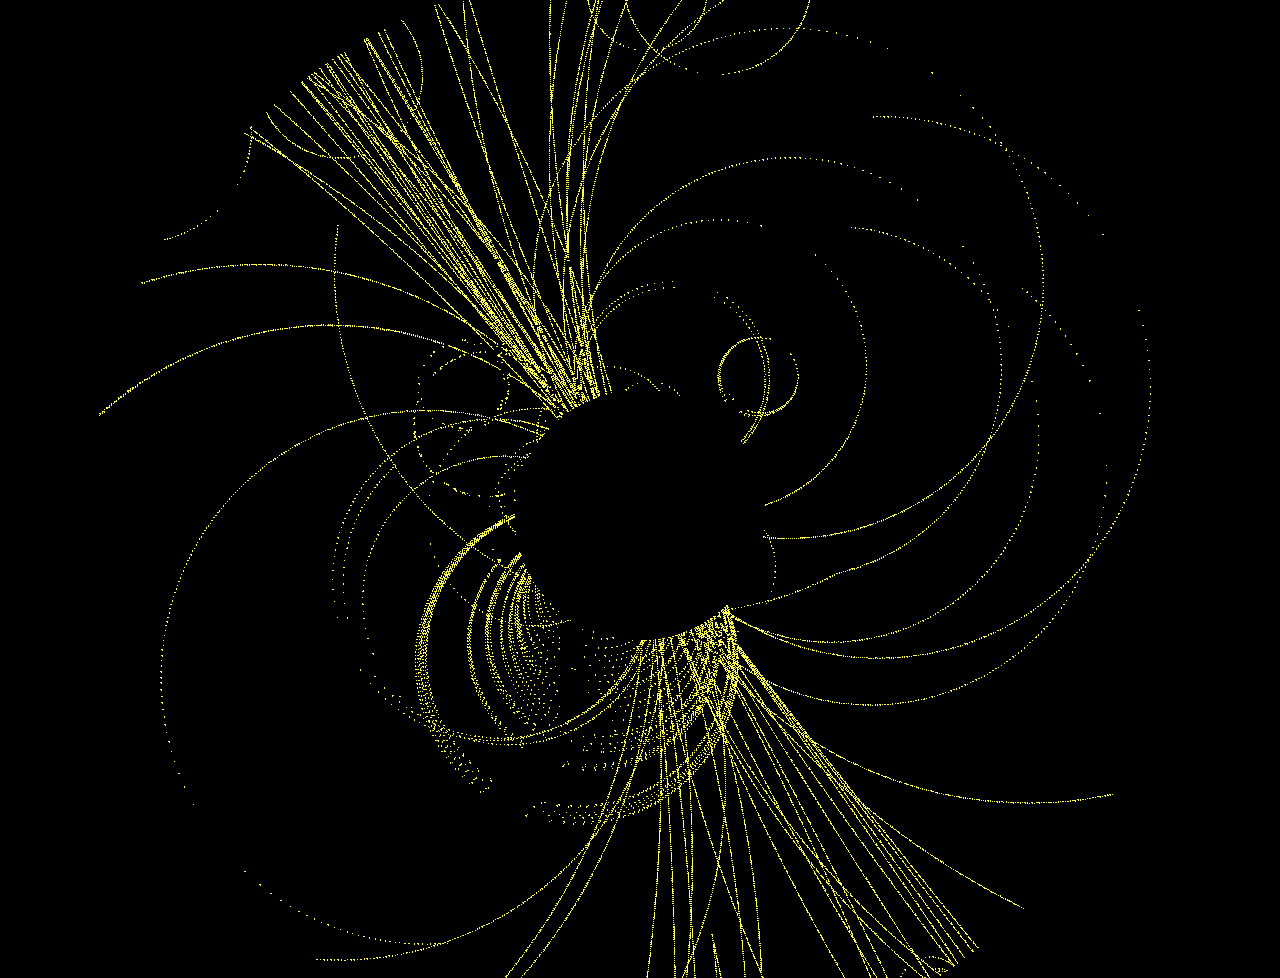
\includegraphics[height=4.4cm]{img/steve_viewer.png}}}
\caption{\label{User viewer}\textsl{User defined}}
\end{minipage}
\end{figure}


%\subsection{CEDViewer}

\section{Shortcuts} 
\label{shortcuts}.


The shortcuts to toggle the visibility of data and detector layers are shown in table \ref{controlshortcuts}, the shortcuts to change settings are listed in table \ref{layershortcuts}.

\begin{center}
\begin{table}
 \begin{tabular}[ht]{|c|l||c|l|}
  \hline
  Shortcut & Option & Shortcut & Option\\
  \hline\hline

$`$ & Toggle visiblity of all data data layers & $\sim$ & Toggle visibility of all detector layers\\
  0 & Toggle data layer 0                  &j   & Toggle detector layer 0\\ 
  1 & Toggle data layer 1                  &k   & Toggle detector layer 1\\ 
  2 & Toggle data layer 2                  &l   & Toggle detector layer 2\\ 
  3 & Toggle data layer 3                  &;   & Toggle detector layer 3\\ 
  4 & Toggle data layer 4                  &`   & Toggle detector layer 4\\ 
  5 & Toggle data layer 5                  &p   & Toggle detector layer 5\\ 
  6 & Toggle data layer 6                  &$[$ & Toggle detector layer 6\\ 
  7 & Toggle data layer 7                  &$]$ & Toggle detector layer 7\\ 
  8 & Toggle data layer 8                  &\textbackslash   & Toggle detector layer 8\\ 
  9 & Toggle data layer 9                  &T   & Toggle detector layer 9\\ 
  ) & Toggle data layer 10                 &Y   & Toggle detector layer 10\\
  ! & Toggle data layer 11                 &U   & Toggle detector layer 11\\
  @ & Toggle data layer 12                 &I   & Toggle detector layer 12\\
  \# & Toggle data layer 13                &O   & Toggle detector layer 13\\
  \$ & Toggle data layer 14                &P   & Toggle detector layer 14\\
  \% & Toggle data layer 15                &$\{$   & Toggle detector layer 15\\
  \textasciicircum  & Toggle data layer 16 &$\}$   & Toggle detector layer 16\\
  \& & Toggle data layer 17                &$|$   & Toggle detector layer 17\\
  $\star$ & Toggle data layer 18           &a   & Toggle detector layer 18\\
  ( & Toggle data layer 19                 &e   & Toggle detector layer 19\\
  t & Toggle data layer 20                 & &\\
  y & Toggle data layer 21                 & &\\
  u & Toggle data layer 22                 & &\\
  i & Toggle data layer 23                 & &\\
  o & Toggle data layer 24                 & &\\
  \hline
\end{tabular}
\caption{Layer shortcuts}
\label{layershortcuts}
\end{table}
\end{center}

\begin{center}
\begin{table}
 \begin{tabular}[ht]{|c|l||c|l|}
  \hline
  Shortcut & Option & Shortcut & Option\\
  \hline\hline
ESC & Quit CED                        &c   & Center object at mouseover          \\ 
h   & Toggle shortcut frame           &Z   & Hold to cut in z-direction          \\ 
r   & reset view                      &z   & Hold to cut in -z-direction         \\ 
R   & Reset CED                       &$>$   & Hold to increase transparency       \\ 
f   & Toggle front view               &$<$   & Hold to decrease transparency       \\ 
s   & Toggle side view                &m   & Hold to increase detector cut angle \\ 
F   & Toggle front projection         &M   & Hold to decrease detector cut angle \\ 
S   & Toggle side projection          &$\leftarrow$  & Move view in z-direction            \\ 
v   & Toggle fisheye projection       &$\rightarrow$  & Move view in -z-direction           \\ 
+   & Zoom in                         &b   & Change background color             \\ 
-   & Zoom out                        & ctrl+z & Undo                            \\                     
\hline
\end{tabular}
\label{controlshortcuts}
\caption{Setting shortcuts}
\end{table}
\end{center}



\section{FAQ}
\subsection{Work with CED from remote}
For a smooth and quick workflow it is always recommended to start CED on the local computer. 
To connect Marlin from a remote computer to your local running CED will be described here.

To allow incoming remote connections, CED must be started with the option 'trust'. The arguments of this option are a hostname or IP address.
\begin{verbatim}
    #On the local computer
    glced -trust <the name of the remote host>
\end{verbatim}
On the computer on which you start Marlin, you need to tell Marlin where to connect to by setting the environment variable CED\_HOST.
\begin{verbatim}
    #On the remote computer
    export CED_HOST=<your local hostname>
    Marlin <your datafile>
\end{verbatim}

\subsection{Change the CED port}
CED binds to a TCP/IP socket to receive data that will be drawn. By default it uses port number 7286. To change it, save the portnumber you want to use in the environment variable CED\_PORT. 
\begin{verbatim}
    export CED_PORT=<Portnumber>
\end{verbatim}
Ensure that the environment variable is set to the same value for Marlin and CED.

\subsection{CED2go}
This tool is designed to enable a quick and simple view into the events of a data file. To start ced2go type:
 \begin{verbatim}
  ced2go <LCIO File>
 \end{verbatim}
Marlin and CED will be started.
\newline\newline
CED2go will determine which gearfile has been used by generating the LCIO file and configure the viewer(s). If you use your very own gearfile you must tell ced2go where to find it, use the -d \textless Gearfile\textgreater   option. The default viewer is the CEDViewer, use the -v option to change it, more than one viewer at the same time is supported. This information has to be written in a XML file to configure Marlin. Secondly ced2go  search for a free TCP/IP port, so its possible to start ced2go several times. After that, CED will start and Marlin connects.
 
%\subsection{Overview}

%\subsection{ced2go options}
%\section{FAQ}

\section{Advanced}
\subsection{Install your own print function}\label{own_picking}
First, the following code has to be inserted into the processEvent function of the viewer (if you use your own viewer):
\begin{verbatim}
CEDPickingHandler &pHandler=CEDPickingHandler::getInstance();
pHandler.update(evt);
\end{verbatim}

The purpose of this code is, that the singleton class CEDPickingHandler knows all objects of the event and therefore assigns a print function for every object. There are predefined default output functions which can be overwritten by the user. To use your own output functions, it is necessary to register them, before calling the update function. That can be done by
calling the register function. The first argument is a collection name or type and the second argument is a pointer to the print function.
Example:
\begin{verbatim}
CEDPickingHandler &pHandler=CEDPickingHandler::getInstance();
pHandler.registerFunction(LCIO::MCPARTICLE, &MyMCParticlePrintFunction);
//...more printfunctions for other types
pHandler.update(evt);
\end{verbatim}

Note: For a proper use of picking, it is essential that the IDs of every object drawn in CED are communicated to CED. This is done by using the functions ced\_line\_ID instead of ced\_line and ced\_hit\_ID instead of ced\_hit. 
\newline
Within the project, print functions have been designed for a number of LCIO objects. The work of Jan Engels served as a basic principle. This allows to send LCIO objects directly to output streams. It is possible to print LCIO objects in a short or long style. The long form:

\begin{verbatim}
Vertex *vertex = (Vertex *) YourLCIOVertexObjekt;
cout << vertex;
\end{verbatim}
The short form:
\begin{verbatim}
Vertex *vertex = (Vertex *) YourLCIOVertexObjekt;
cout << lc_short(vertex);
\end{verbatim}
The short form allows to print objects as tables:
\begin{verbatim}
Vertex *vertex1 = (Vertex *) YourLCIOVertexObjekt1;
Vertex *vertex2 = (Vertex *) YourLCIOVertexObjekt2;
cout << header(vertex) << tail(vertex) << lcshort(vertex1) << lcshort(vertex2)
<< tail(vertex);
\end{verbatim}
or:
\begin{verbatim}
cout << header(EVENT::Vertex) << tail(EVENT::Vertex) << lcshort(vertex1)
<< lcshort(vertex2) << tail(EVENT::Vertex);
\end{verbatim}
This method of printing is available for the following LCIO types: MCParticle, TrackerHit,
SimTrackerHit, CalorimeterHit, SimCalorimeterHit, ReconstructedParticle, Track and Cluster.

\subsection{MarlinUtil::MarlinCED}
MarlinUtil::MarlinCED is a library used by Marlin, which provides the functions to draw data into CED. This function simply calls the ced draw functions. It also provides the client part of picking, which means the  mapping between LCIO objects and LCIO ID, and calling the output function of the selected object. For details of the picking part see chapter \ref{own_picking}.


\subsection{Advanced configuration}
Additional options are avaiable in the config file \textit{ced\_config.h} it is nesessary to compile CED again after changes.

\subsection{User defined client}
\label{myviewer}
You are able to create your own CED client for special use cases.  

An example for a simple client written in C++ is:
\begin{verbatim}
#include <iostream>
#include <vector>
#include "ced_cli.h"
using namespace std;

int main(void){
    ced_client_init("localhost",7286);
    ced_register_elements();

    ced_new_event();

    unsigned yellow=0xf5f300;
    unsigned green=0x7bf300;
    unsigned blue=0x4949dd;
    unsigned grey=0xabaaab;
    unsigned violett=0x651c93;
    unsigned red=0xff0000;

    unsigned layer_detec1=25;
    unsigned layer_detec2=26;

    unsigned layer_data1=1;
    unsigned layer_data2=2;

    //draw detector:
    std::vector<CEDGeoTube> gTV ;
    gTV.push_back(CEDGeoTube(10000, 10500,  4, 4,  0, 0, 10000, -10000, 
         violett, layer_detec1, 0,0));
    gTV.push_back(CEDGeoTube(1500,   4000, 30, 4,  0, 0, 10000, -10000, 
         blue, layer_detec2,    0,0));
    gTV.push_back(CEDGeoTube(7000,   7150,  4, 4, 45, 0, 10000, -10000, 
         yellow, layer_detec2,  0,0));
    gTV.push_back(CEDGeoTube(11000, 11500,  4, 4,  0, 0, 10000, -10000, 
         red, layer_detec2,     0,0));
    ced_geotubes( gTV.size() ,  (CED_GeoTube*) &gTV[0] );

    ced_describe_layer("Example detector 1", layer_detec1 );
    ced_describe_layer("Example detector 1", layer_detec2 );

    ced_hit_ID(-11000.,-11000.,0., 0, layer_data1, grey,1);
    ced_hit_ID( 11000.,-11000.,0., 0, layer_data1, grey,2);
    ced_hit_ID(-11000., 11000.,0., 0, layer_data1, grey,3);
    ced_hit_ID( 11000., 11000.,0., 0, layer_data1, grey,40);
    ced_describe_layer("Data layer 1", layer_data1 );

    ced_line_ID( 0, 0, 0, -10000, -10000,  0, 1 , layer_data2, green, 5);
    ced_line_ID( 0, 0, 0, -10000,  10000,  0, 1 , layer_data2, green, 6);
    ced_line_ID( 0, 0, 0,  10000, -10000,  0, 1 , layer_data2, green, 7);
    ced_line_ID( 0, 0, 0,  10000,  10000,  0, 1 , layer_data2, green, 8);
    ced_describe_layer("Data layer 2", layer_data2 );

    ced_send_event();
\end{verbatim}

Compile this programm (for example) with:
\begin{verbatim}
  export LD_LIBRARY_PATH=/path/to/CED/lib/
  gcc -I /path/to/ced/src/include/ -o test test.cc -L /path/to/CED/build/lib/ -l CED
\end{verbatim}

Run CED and start this new programm
\begin{verbatim}
  glced& 
  ./test
\end{verbatim}
The output is shown in figure \ref{myviewer_pic}.
\begin{figure}
    \begin{center}
         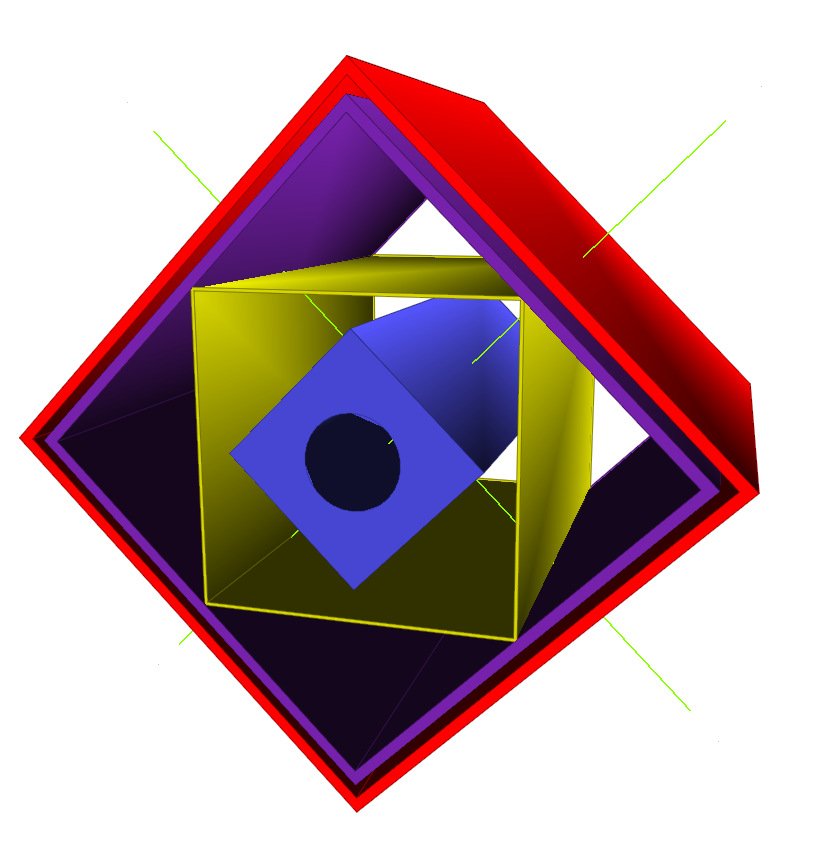
\includegraphics[width=0.8\linewidth]{img/example_viewer.png}
         \caption{\label{myviewer_pic} \textsl{The output of the example client}}
    \end{center}
\end{figure}


Of course you are able to run the client as a CERN-ROOT macro. 
The important step is that root need to know the CED library

\begin{verbatim}
  {
    gSystem->Load("libCED");
    gROOT->ProcessLine(".L your_program.C+");
    your_function();
}
\end{verbatim}



\end{document}
